\documentclass[../main.tex]{subfiles}
\graphicspath{{img},{img/ink},{ink}}

\begin{document}

\begin{tcolorbox}[
    width=\textwidth,
    height=\textheight,
    title=Phyphox: Fadenpendel,
    fonttitle=\Large,
    before title=\vspace{0.2cm}, after title=\vspace{0.2cm},
    colback=white,
    title filled=true, 
    colbacktitle=myorange,
    colframe=black,
    coltitle=black,
    ]

    \vspace{0.2cm}
    \begin{minipage}[]{0.75\textwidth}

        \textbf{Klassenstufe}: 9/10 (qualitativ), 11/12 (DGL)

        \vspace{0.5cm}

        \textbf{Fachlicher Bezug}: Pendelbewegung, Schwingung, Bestimmung von Einflussgrößen, Formel der Periodendauer

        \vspace{0.5cm}
        \textbf{Material}: Stativmaterial, Schnur, Holzstücke, Halterung, Handy + Phyphox

        \vspace{0.5cm}
        \textbf{Aufbau}: Die Halterung des Federpendels lässt sich auch hier verwenden. Es reicht eine Schnur aus, die Laschen in verschiedenen Abständen enthält. Dadurch lassen sich später schnell verschiedene Schwingungslängen einstellen. Zusätzliche Holzstücke lassen sich an der Unterseite der Halterung durch Gummibänder anbringen. 
    \end{minipage}
    \hspace{0.6cm}
    \begin{minipage}[]{0.2\textwidth}
        \includegraphics[width=0.95\textwidth]{img/versuchsaufbau}
    \end{minipage}

    \vspace{0.5cm}
    \begin{minipage}[]{0.75\textwidth}
        \textbf{Durchführung}: Bei der Schwingung erfolgt eine Rotation um die y-Achse. In der Phyphox-App eigenet sich deshalb die Betrachtung der y-Komponente des Gyroskops. Der Fernzugriff wird ggf. aktiviert. Die SuS untersuchen die Abhängigkeit der Periodendauer $T$ von 
        \begin{itemize}[noitemsep]
            \item verschiedenen Auslenkungungen $x$ des Pendel
            \item der Masse $m$ des Schwingers 
            \item verschiedene Längen $l$ der Schnur
        \end{itemize}
        Die Ergebnisse werden in eine Tabelle eingetragen. Die zusätzliche Berechnung der Größe $\sqrt{l}$ wird vorgegeben.

    \end{minipage}
    \hspace{0.1cm}
    \begin{minipage}[]{0.2\textwidth}
        \includegraphics[width=1.1\textwidth]{img/app}
    \end{minipage}
    
    \vspace{0.5cm}
    \textbf{Ergebnis}: Die Periodendauer $T$ ist unabhängig von der Auslenkung $x$ zu Beginn und der Masse $m$ des schwingenden Objekts. Man beobachtet die Proportionalität.
    \begin{align*}
        T \sim \sqrt{l} 
    \end{align*}
    Aus einer Messung kann man durch Vorgabe der Formel $T=2 \pi \sqrt{\frac{l}{g}}$ den Wert der Erdbeschleunigung 
    \begin{align*}
        g = l \cdot \left(\frac{2\pi}{T}\right)^2
    \end{align*}
    bestimmen.


    \vspace{0.5cm}
    \textbf{Didaktische Bemerkungen}: Zur Kontrolle oder nachdem die SuS eigene Beobachtungen gemacht haben, kann in der Phyphox-App unter dem Reiter \glqq Mechanik \grqq{} die Auswahl \glqq Fadenpendel \grqq{} getroffen werden. Dort werden die Berechnungen von der Software durchgeführt.\\
    Die Konstruktion einer Halterung (eigene Idee der SuS) und Durchführung des Experiments bietet sich auch als Hausaufgabe an.

\end{tcolorbox}


\end{document}
